\documentclass[MusicXML.tex]{subfiles}

\newpage
\begin{document}
\section{MusicXML Online Application}

The purpose of this application is to offer a platform where users can convert their music XML files to sheet music and sound and extract useful information. This way they can listen to the music and also search through its contents. This section describes the application’s architecture and the results of the experiment. In conclusion, some future extensions to the application are also described.

\subsection{Architecture}
The application is built as a web application using Java (JDK 1.7). When XML files are uploaded, the musicxml2ly command is automatically executed on the command line to convert the XML file to a lilypond (.ly) file. Once completed, the command line version of Lilypond is invoked to convert the .ly file to a pdf and a MIDI-audio file. 
The backend of the application consists of three classes described below:

\begin{itemize}
\item Exist - Database wrapper which handles connecting to the database, uploading XML files to the database and executing queries. Most of this code was taken from the textbook and/or the eXist website and then slightly modify to suit the specific needs of the application.

\item XMLFileUploadServlet - This servlet deals with the heavy lifting around uploading files. After an uploaded file is saved on disk the servlet also uploads the content of the XML file to the eXist database (using Exist.java). It also immediately converts the .xml file to an audio file and a pdf.

\item MusicXMLOnline - Being the backbone of the application, the MusicXMLOnline class offers functions to retrieve all documents and documentTitles, to extract the lyrics from a document and to search the lyrics and titles of the songs in the database.
 
\end{itemize}

To deliver all user content, .jsp files are used. The first jsp file is used for displaying the available files and search results, the second one to upload the files, and the third file handles the case where users can listen to the music and read the lyrics. To easily create a powerful user experience that works on mobile phones as well as traditional browsers, the bootstrap framework is used.

\subsection{Results}
After working hard on the application, the basic functionality that was planned was also completed. It is possible for users to upload and convert XML files, search through these files, view the sheet music, and also listen to the music while reading the lyrics. 

As can be seen from the Figures \ref{fig:musicindex} and \ref{fig:musicpdf} the functionality for displaying an overview of the songs and the sheet music works exactly as expected. 

\begin{figure} [H]
	\centering
	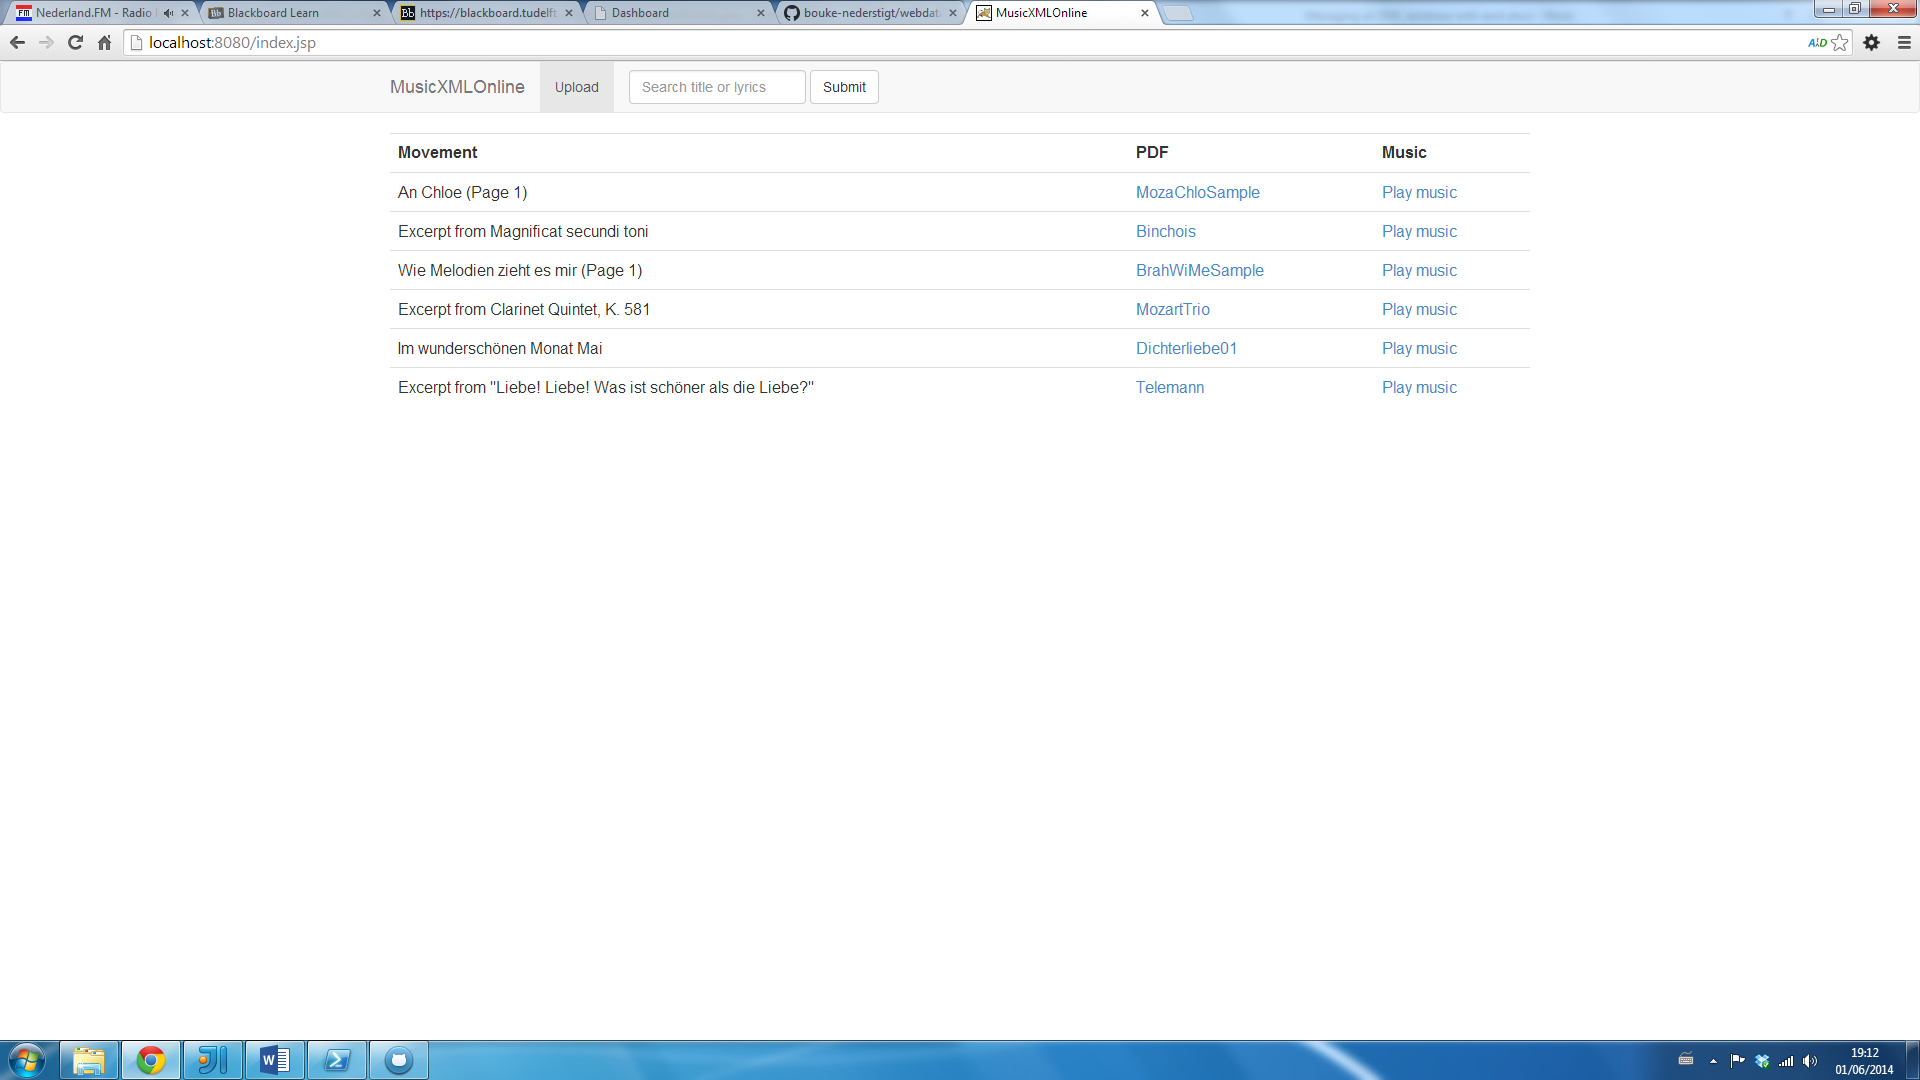
\includegraphics[width=1\textwidth]{./Figures/MusicXMLOnline-index.png}
	\caption{Music Online Contents Page}
	\label{fig:musicindex}
\end{figure}

\begin{figure} [H]
	\centering
	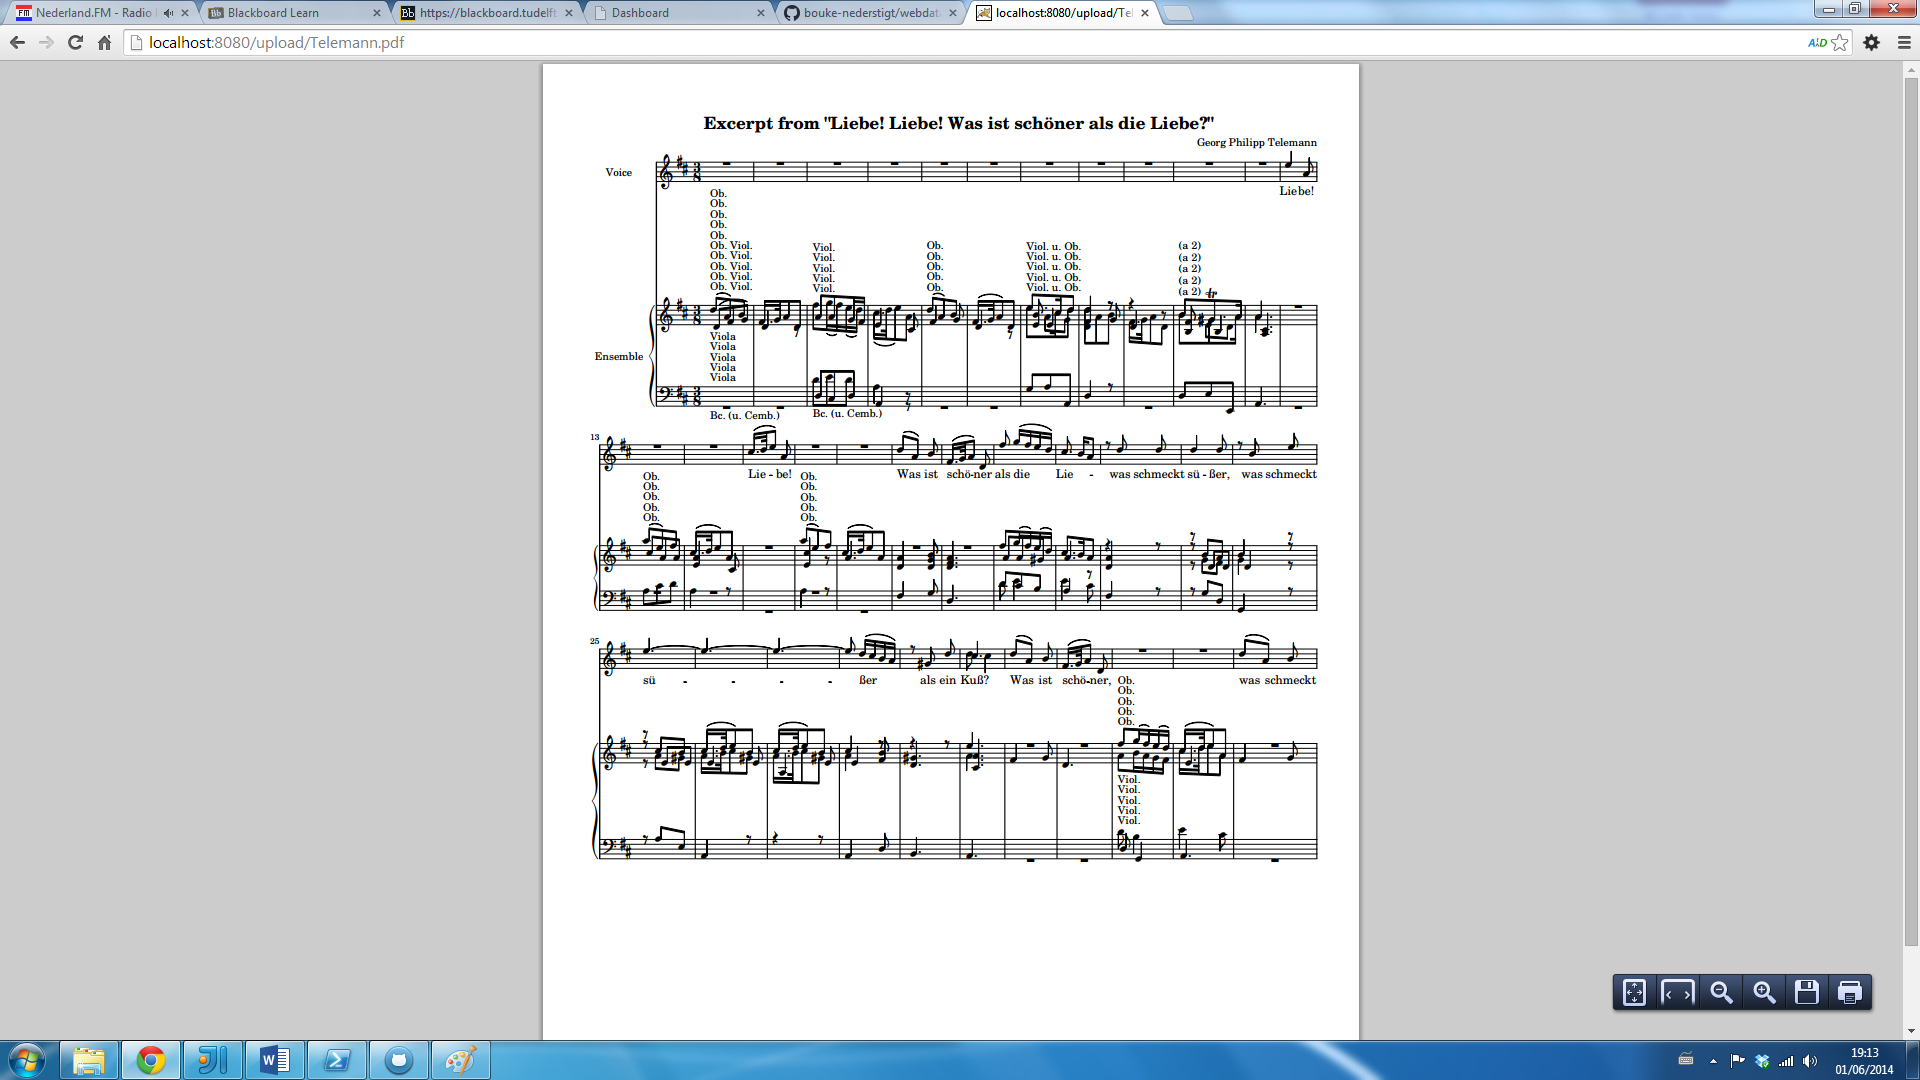
\includegraphics[width=1\textwidth]{./Figures/MusicXMLOnline-pdf.png}
	\caption{Additional Movie Information}
	\label{fig:musicpdf}
\end{figure}

The functionality for displaying the lyrics and searching through the songs is however slightly more limited. There are two main drawbacks that are described below:  

\begin{enumerate}
\item The search functionality is quite rudimentary. When a user searches for a string and all the words in the string are found in either the lyrics, or the title the song is returned. A better search function would however also keep in mind thinks like capitalization, or offer the possibility to combine words from the title and lyrics. It could also be possible to include e.g. author information. The output results are shown in Figure \ref{fig:musiclyricssearch}.

\begin{figure} [H]
	\centering
	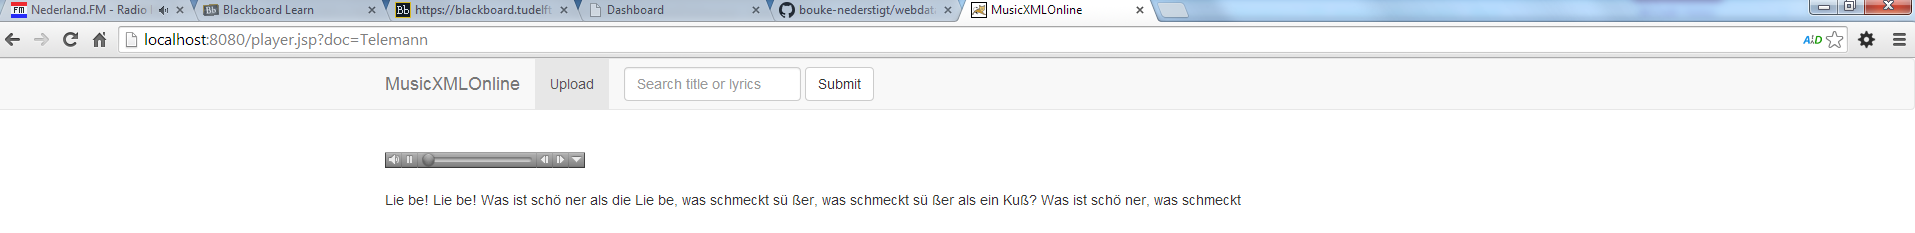
\includegraphics[width=1\textwidth]{./Figures/MusicXMLOnline-player.png}
	\caption{Song Lyrics Search}
	\label{fig:musiclyricssearch}
\end{figure}

\item All of the lyrics are retrieved from the database, but the words are not always put together correctly. Because the words are sometimes split over different notes they are not always retrieved in one piece - Figure \ref{fig:musicpdf} shows this problem.

\begin{figure} [H]
	\centering
	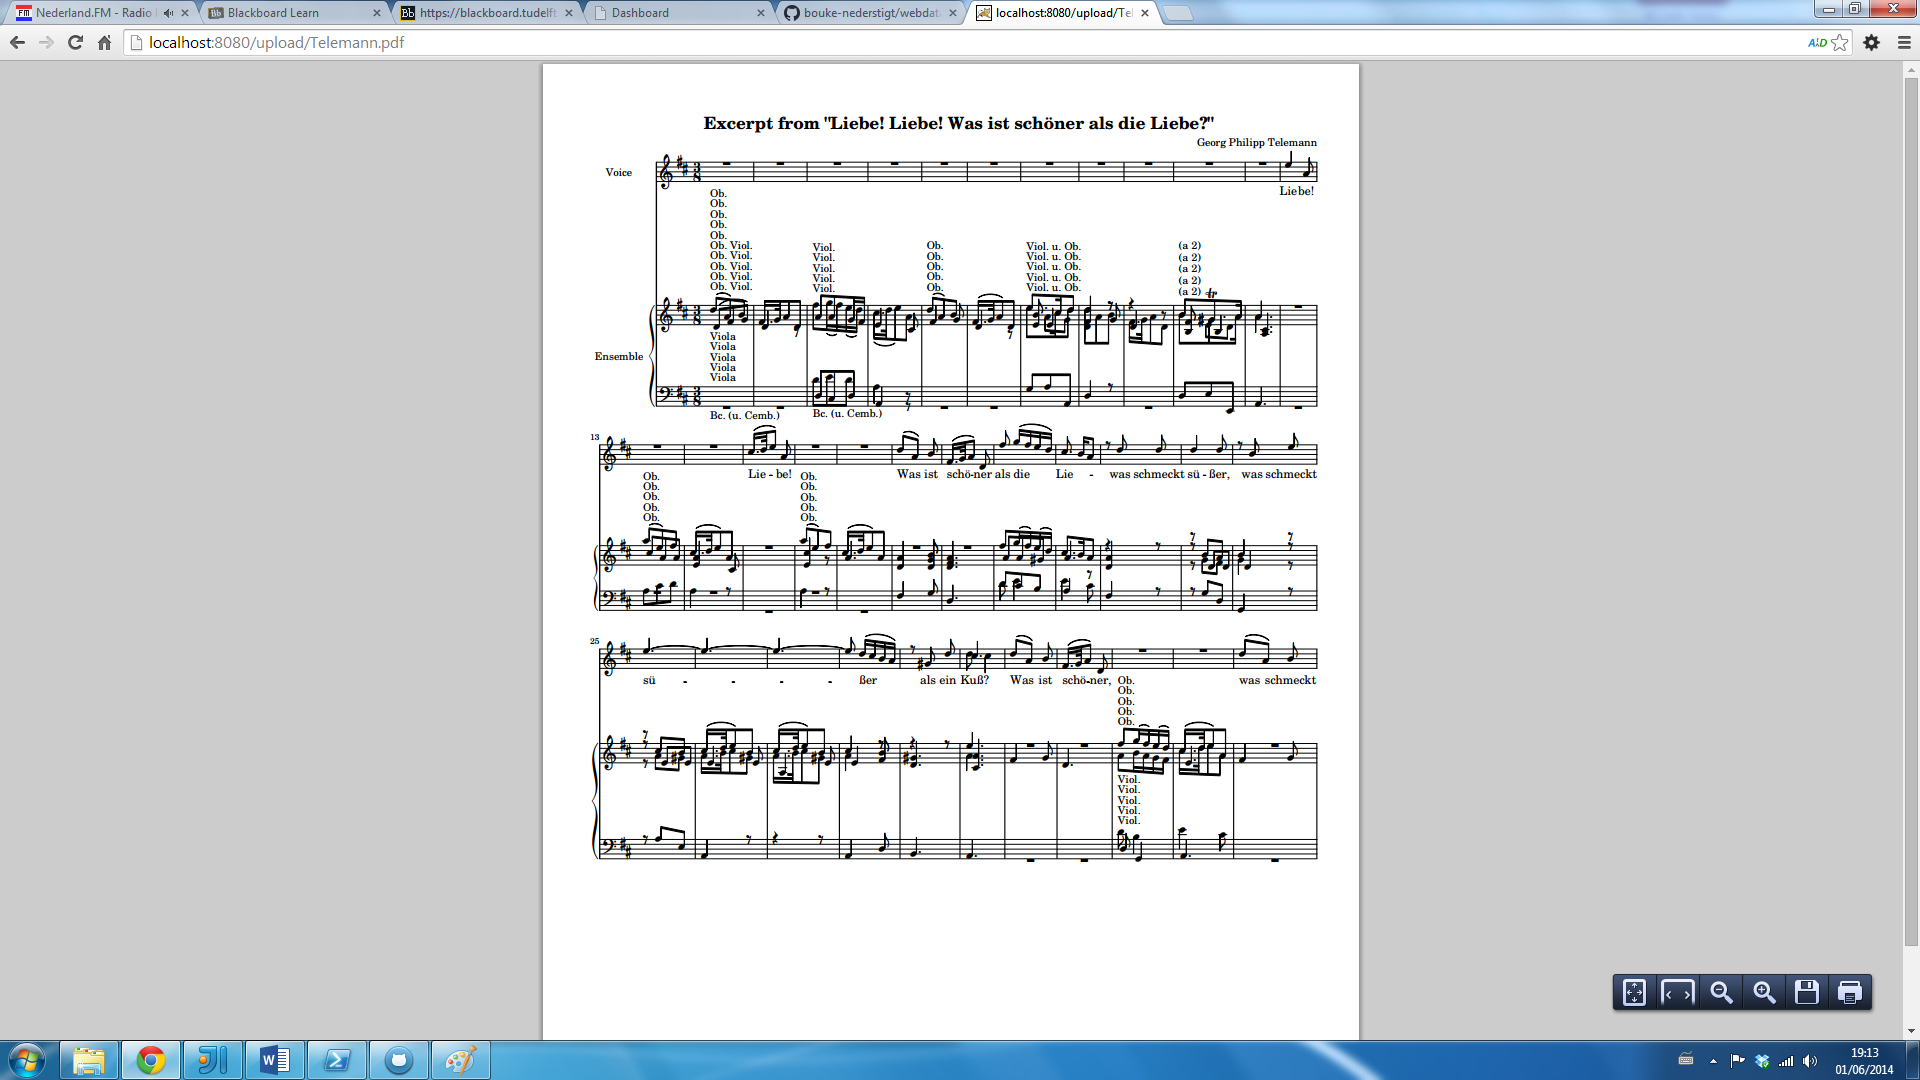
\includegraphics[width=1\textwidth]{./Figures/MusicXMLOnline-pdf.png}
	\caption{Additional Movie Information}
	\label{fig:musicpdf}
\end{figure}

\end{enumerate}
\end{document}